\documentclass{article}
\usepackage{graphicx}
\usepackage[brazilian]{babel}
\usepackage[utf8]{inputenc}
\usepackage[T1]{fontenc}
\usepackage{amsmath}
\usepackage{amssymb}
\setlength{\parindent}{0in}
\usepackage{hyperref}

\begin{document}
	
	\title{Provinha 07 - MAE0119}
	\author{Daniel Yoshio Hotta – 9922700}
	
	\maketitle	
	
		Enviado termo geral.
	
	\textbf {E.a.} 
	\\ \\
	\textit {Resposta:} \\
	
	Usei o desmos para ilustrar após fazer na mão. 
    
    \begin{figure}[h]
    	\caption{Exercício a.}
    	\centering % para centralizarmos a figura
    	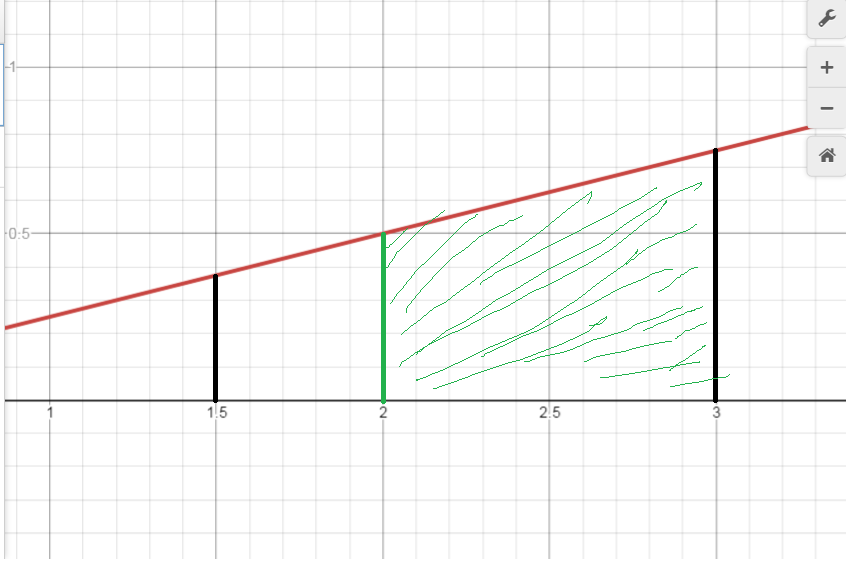
\includegraphics[width=10cm]{a.png} % leia abaixo
    	\label{figura:ex.a}
    \end{figure}

    Temos o gráfico da função densidade de probabilidade e notamos que, nos pontos (1.5, 0.375), (2, 0.5) e (3, 0.75), a linearidade da função nos permite deduzir que ao considerarmos somente os valores de $Y \geq 1.5$, o ponto (2, 0.5) divide a probabilidade em exatos 1/3 para a esquerda e 1/3 para a direita. Logo:\\

    $P(Y>2 | Y \geq 1.5) = 2/3$
    
    \textbf {E.b.} 
    \\ \\
    \textit {Resposta:} \\
    
    
	
	
	
\end{document}
